
\begin{figure}
\centering

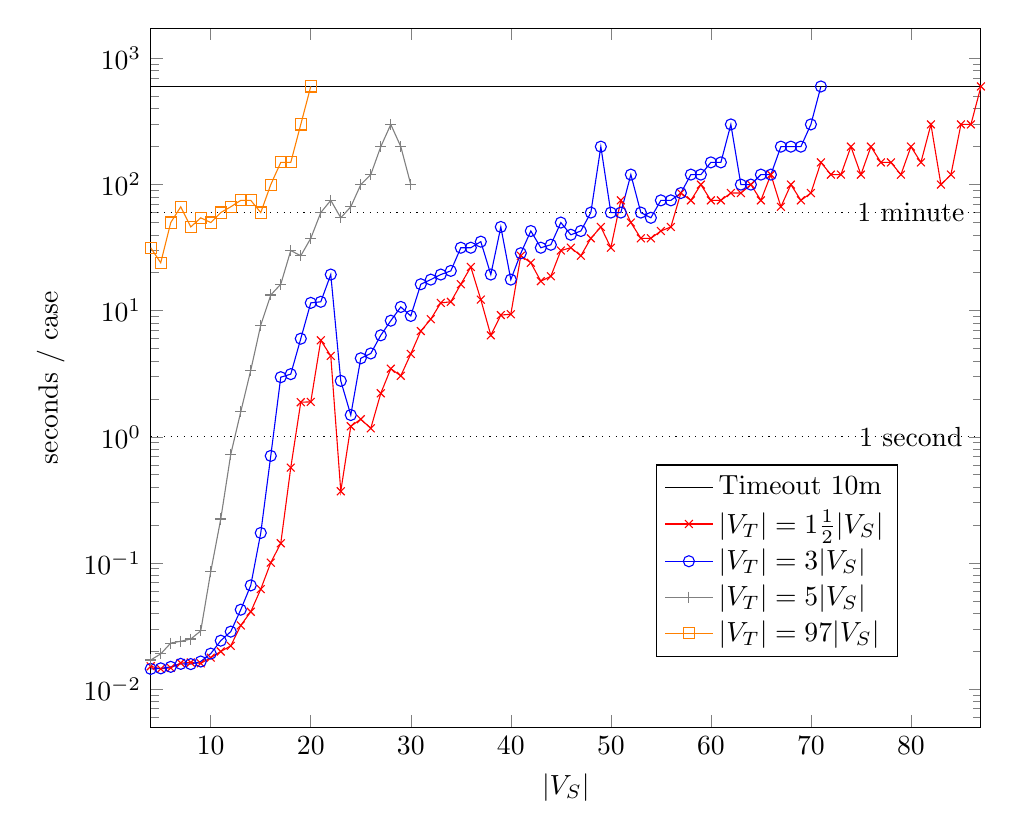
\begin{tikzpicture}
    \begin{axis}[
        xlabel=$|V_S|$,
        ylabel=seconds / case,
        ymode=log,
        legend style={at={(0.9,0.1)},anchor=south east},
        width=\textwidth,
        legend cell align={left},
        xmin=4,
        xmax=87,
    ]
    
    \addplot[
        mark=none,
        black,
    ] plot coordinates {
        (4,600)
        (87,600)
};
    \addlegendentry{Timeout 10m} 
    
        \addplot[
        mark=none,
        black,
        dotted,
        forget plot,
    ] plot coordinates {
        (4,1)
        (87,1)
};
      \addplot[
        mark=none,
        black,
        dotted,
        forget plot,
    ] plot coordinates {
        (4,60)
        (87,60)
};
    \node[] at (axis cs: 80,1) {1 second};
    \node[] at (axis cs: 80,60) {1 minute};


    \addplot[
        mark=x,
        red,
    ] plot coordinates {
        (4,0.015145145145145146)
        (5,0.014459)
        (6,0.014727)
        (7,0.016091)
        (8,0.016229)
        (9,0.015978)
        (10,0.01773)
        (11,0.019843)
        (12,0.021997)
        (13,0.031924)
        (14,0.041004)
        (15,0.061994999999999995)
        (16,0.10044744744744744)
        (17,0.14312200000000003)
        (18,0.569784)
        (19,1.8808777429467085)
        (20,1.8927444794952681)
        (21,5.825242718446602)
        (22,4.37956204379562)
        (23,0.370036)
        (24,1.2121212121212122)
        (25,1.3793103448275863)
        (26,1.1673151750972763)
        (27,2.2140221402214024)
        (28,3.468208092485549)
        (29,3.045685279187817)
        (30,4.545454545454546)
        (31,6.896551724137931)
        (32,8.571428571428571)
        (33,11.538461538461538)
        (34,11.764705882352942)
        (35,16.216216216216218)
        (36,22.22222222222222)
        (37,12.244897959183673)
        (38,6.382978723404255)
        (39,9.23076923076923)
        (40,9.375)
        (41,27.272727272727273)
        (42,24.0)
        (43,17.142857142857142)
        (44,18.75)
        (45,30.0)
        (46,31.57894736842105)
        (47,27.272727272727273)
        (48,37.5)
        (49,46.15384615384615)
        (50,31.57894736842105)
        (51,75.0)
        (52,50.0)
        (53,37.5)
        (54,37.5)
        (55,42.857142857142854)
        (56,46.15384615384615)
        (57,85.71428571428571)
        (58,75.0)
        (59,100.0)
        (60,75.0)
        (61,75.0)
        (62,85.71428571428571)
        (63,85.71428571428571)
        (64,100.0)
        (65,75.0)
        (66,120.0)
        (67,66.66666666666667)
        (68,100.0)
        (69,75.0)
        (70,85.71428571428571)
        (71,150.0)
        (72,120.0)
        (73,120.0)
        (74,200.0)
        (75,120.0)
        (76,200.0)
        (77,150.0)
        (78,150.0)
        (79,120.0)
        (80,200.0)
        (81,150.0)
        (82,300.0)
        (83,100.0)
        (84,120.0)
        (85,300.0)
        (86,300.0)
        (87,600.0)
    };
    \addlegendentry{$|V_T|=1\frac{1}{2}|V_S|$}
    
    
\addplot[
        mark=o,
        blue,
    ] plot coordinates {
        (4,0.014433999999999999)
        (5,0.014587)
        (6,0.014992)
        (7,0.015832000000000002)
        (8,0.01576)
        (9,0.01653)
        (10,0.019097000000000003)
        (11,0.024178)
        (12,0.028518)
        (13,0.042565)
        (14,0.066355)
        (15,0.172921)
        (16,0.7058823529411765)
        (17,2.9702970297029703)
        (18,3.141361256544503)
        (19,6.0)
        (20,11.538461538461538)
        (21,11.764705882352942)
        (22,19.35483870967742)
        (23,2.7777777777777777)
        (24,1.488833746898263)
        (25,4.195804195804196)
        (26,4.580152671755725)
        (27,6.382978723404255)
        (28,8.333333333333334)
        (29,10.714285714285714)
        (30,9.090909090909092)
        (31,16.216216216216218)
        (32,17.647058823529413)
        (33,19.35483870967742)
        (34,20.689655172413794)
        (35,31.57894736842105)
        (36,31.57894736842105)
        (37,35.294117647058826)
        (38,19.35483870967742)
        (39,46.15384615384615)
        (40,17.647058823529413)
        (41,28.571428571428573)
        (42,42.857142857142854)
        (43,31.57894736842105)
        (44,33.333333333333336)
        (45,50.0)
        (46,40.0)
        (47,42.857142857142854)
        (48,60.0)
        (49,200.0)
        (50,60.0)
        (51,60.0)
        (52,120.0)
        (53,60.0)
        (54,54.54545454545455)
        (55,75.0)
        (56,75.0)
        (57,85.71428571428571)
        (58,120.0)
        (59,120.0)
        (60,150.0)
        (61,150.0)
        (62,300.0)
        (63,100.0)
        (64,100.0)
        (65,120.0)
        (66,120.0)
        (67,200.0)
        (68,200.0)
        (69,200.0)
        (70,300.0)
        (71,600.0)
};
    \addlegendentry{$|V_T|=3|V_S|$}
   
\addplot[
        mark=+,
        gray,
    ] plot coordinates {
            (4,0.016998998998999)
        (5,0.018996)
        (6,0.023146)
        (7,0.023915)
        (8,0.024909)
        (9,0.028915)
        (10,0.085258)
        (11,0.22293700000000002)
        (12,0.7263922518159807)
        (13,1.5789473684210527)
        (14,3.3707865168539324)
        (15,7.6923076923076925)
        (16,13.333333333333334)
        (17,16.216216216216218)
        (18,30.0)
        (19,27.272727272727273)
        (20,37.5)
        (21,60.0)
        (22,75.0)
        (23,54.54545454545455)
        (24,66.66666666666667)
        (25,100.0)
        (26,120.0)
        (27,200.0)
        (28,300.0)
        (29,200.0)
        (30,100.0)

};
    \addlegendentry{$|V_T|=5|V_S|$}
    
 \addplot[
        mark=square,
        orange,
    ] plot coordinates {
        (4,31.57894736842105)
        (5,24.0)
        (6,50.0)
        (7,66.66666666666667)
        (8,46.15384615384615)
        (9,54.54545454545455)
        (10,50.0)
        (11,60.0)
        (12,66.66666666666667)
        (13,75.0)
        (14,75.0)
        (15,60.0)
        (16,100.0)
        (17,150.0)
        (18,150.0)
        (19,300.0)
        (20,600.0)
};
     \addlegendentry{$|V_T|=97|V_S|$}

    \end{axis}
    \end{tikzpicture}


\caption{Performance of our algorithm $\mathit{RTSH}$ using the configurations that individually perform best: DFS path iteration, avoiding unnecessarily long paths and N-reachability AllDifferent pruning. Contraction is disabled. We use 10 minutes worth of tests for each data point and stop testing when that is not enough for finding a homeomorphism in a single test case.}
\label{fig:highperformance}
\end{figure}
